\documentclass[11pt,a4paper]{article}
\usepackage{amsmath,amssymb,amsfonts}
\usepackage{booktabs}
\usepackage{geometry}
\usepackage{hyperref}
\usepackage{enumitem}
\usepackage{xcolor}
\usepackage{listings}
\usepackage{mathtools}
\usepackage{tikz}
\usepackage{float}
\usepackage{caption}
\usepackage{subcaption}
\usepackage{longtable}
\usepackage{multirow}
\usepackage{array}

\usetikzlibrary{arrows.meta, positioning, shapes.geometric, fit, calc, decorations.pathreplacing}

\geometry{margin=0.9in}

\newcommand{\Zq}{\mathbb{Z}_{3329}}
\newcommand{\brev}[1]{\operatorname{BitRev}_{7}\!\left(#1\right)}
\newcommand{\modinv}[1]{#1^{-1}}
\newcommand{\modneg}[1]{\widetilde{#1}}
\newcommand{\sv}[1]{\texttt{#1}}
\newcommand{\port}[1]{\texttt{#1}}
\newcommand{\rom}[1]{\textsc{#1}}

\definecolor{nttblue}{RGB}{41,98,163}
\definecolor{inttred}{RGB}{180,40,40}
\definecolor{cwmgreen}{RGB}{40,140,60}
\definecolor{codebg}{RGB}{245,245,245}

\lstset{
    language=Verilog,
    basicstyle=\ttfamily\small,
    keywordstyle=\color{nttblue}\bfseries,
    commentstyle=\color{gray}\itshape,
    backgroundcolor=\color{codebg},
    frame=single,
    breaklines=true,
    columns=fullflexible,
    morekeywords={logic,always_ff,always_comb,localparam,assign,import,module,endmodule,input,output,typedef,enum,case,endcase,begin,end,parameter}
}

\title{%
  \textbf{Twiddle Factor ROM \& Address Generator}\\[0.3em]
  \large Hardware Architecture, Mathematical Derivation, and Usage Guide\\[0.3em]
  \normalsize For the ML-KEM Mixed-Radix-4/2 NTT/INTT Accelerator
}
\author{Poly-Arith-Unit Project $\cdot$ Inha University UniPAM Architecture}
\date{March 2026}

\begin{document}
\maketitle
\tableofcontents
\newpage

% #########################################################################
\part{Mathematical Foundations}
% #########################################################################

% =====================================================================
\section{The Arithmetic Field}
% =====================================================================

All operations are performed in the prime field $\Zq$, where
\begin{equation}
  q = 3329
\end{equation}
is the ML-KEM (FIPS~203) modulus. Every element $a \in \Zq$ satisfies $0 \le a < 3329$ and can be represented in 12~bits ($\lceil \log_2 3329 \rceil = 12$).

\paragraph{Field operations.}
\begin{alignat}{2}
  a + b   &\;\triangleq\; (a + b) &&\bmod q \\
  a - b   &\;\triangleq\; (a - b + q) &&\bmod q \\
  a \cdot b &\;\triangleq\; (a \times b) &&\bmod q
\end{alignat}

% =====================================================================
\section{Primitive Root of Unity}
% =====================================================================

\subsection{Definition}

The Number Theoretic Transform of length $N = 256$ over $\Zq$ requires a primitive $N$-th root of unity $\zeta$ such that:
\begin{align}
  \zeta^{N} &\equiv 1 \pmod{q} \label{eq:root-unity}\\
  \zeta^{k} &\not\equiv 1 \pmod{q} \quad \text{for all } 0 < k < N \label{eq:primitive}
\end{align}

For ML-KEM, the standard choice is:
\begin{equation}
  \boxed{\zeta = 17}
\end{equation}

\paragraph{Verification.}
$17^{256} \bmod 3329 = 1$, and $\text{ord}(17) = 256$ in $\mathbb{Z}_{3329}^{*}$.

\subsection{The Power Table}

Define:
\begin{equation}
  \zeta^{[k]} \triangleq 17^{k} \bmod 3329, \qquad k = 0, 1, \ldots, 255
\end{equation}

Computed iteratively:
\begin{equation}
  \zeta^{[0]} = 1, \qquad \zeta^{[k]} = \zeta^{[k-1]} \cdot 17 \bmod 3329
\end{equation}

% =====================================================================
\section{The 7-Bit Bit-Reversal Permutation}
% =====================================================================

\subsection{Definition}

For a 7-bit integer $v = (b_6\, b_5\, b_4\, b_3\, b_2\, b_1\, b_0)_2$:
\begin{equation}
  \brev{v} = (b_0\, b_1\, b_2\, b_3\, b_4\, b_5\, b_6)_2
  \label{eq:bitrev-def}
\end{equation}

\subsection{Key Property: Involution}

Bit-reversal is its own inverse:
\begin{equation}
  \brev{\brev{v}} = v \qquad \forall\, v \in \{0, 1, \ldots, 127\}
  \label{eq:involution}
\end{equation}

\subsection{Worked Examples}

\begin{center}
\begin{tabular}{ccc}
\toprule
$v$ (decimal) & $v$ (7-bit binary) & $\brev{v}$ \\
\midrule
$0$  & $0000000$ & $0 $  \\
$1$  & $0000001$ & $64$  \\
$2$  & $0000010$ & $32$  \\
$3$  & $0000011$ & $96$  \\
$64$ & $1000000$ & $1 $  \\
$127$& $1111111$ & $127$ \\
\bottomrule
\end{tabular}
\end{center}

% =====================================================================
\section{The FIPS-Style ZETA Table}
\label{sec:zeta-table}
% =====================================================================

Following ML-KEM (FIPS~203), the base twiddle factor lookup table has 128 entries:
\begin{equation}
  \boxed{ZETA[i] = \zeta^{\,\brev{i}} \bmod q, \qquad i = 0, 1, \ldots, 127}
  \label{eq:zeta-table}
\end{equation}

\paragraph{The double-reversal access identity.}
When we access the table with a bit-reversed index:
\begin{equation}
  ZETA\!\left[\brev{x}\right] = \zeta^{\,\brev{\brev{x}}} = \zeta^{x} \bmod q
  \label{eq:access-identity}
\end{equation}

This is the fundamental identity that allows us to recover any desired power $\zeta^x$ from the FIPS-style table.

\paragraph{Verification of key entries:}
\begin{align*}
  ZETA[0]  &= \zeta^{\brev{0}}  = \zeta^{0}  = 1 \\
  ZETA[1]  &= \zeta^{\brev{1}}  = \zeta^{64} = 1729 \\
  ZETA[64] &= \zeta^{\brev{64}} = \zeta^{1}  = 17
\end{align*}

% =====================================================================
\section{Modular Inverse via Fermat's Little Theorem}
\label{sec:fermat}
% =====================================================================

Since $q = 3329$ is prime, Fermat's Little Theorem gives us:
\begin{equation}
  a^{q-1} \equiv 1 \pmod{q} \quad \text{for } a \not\equiv 0
\end{equation}

Therefore the modular multiplicative inverse is:
\begin{equation}
  \boxed{a^{-1} \equiv a^{q-2} \equiv a^{3327} \pmod{3329}}
  \label{eq:fermat-inv}
\end{equation}

\paragraph{Example: The fourth root of unity.}
\begin{align*}
  \omega_4 &= \zeta^{N/4} = \zeta^{64} = 17^{64} \bmod 3329 = 1729 \\
  \omega_4^{-1} &= 1729^{3327} \bmod 3329 = 1600
\end{align*}

Verify: $1729 \times 1600 \bmod 3329 = 2766400 \bmod 3329 = 1$. $\checkmark$

% =====================================================================
\section{The Pre-Negation Trick (INTT Hardware Optimization)}
\label{sec:pre-negate}
% =====================================================================

\subsection{The Problem: Sign Mismatch}

The FIPS~203 inverse NTT butterfly (Algorithm~10) requires:
\begin{equation}
  V_{\text{FIPS}} = \zeta^{-1} \cdot (a_{\text{bot}} - a_{\text{top}}) \bmod q
  \label{eq:fips-butterfly}
\end{equation}

However, our Processing Elements are hardwired to compute:
\begin{equation}
  V_{\text{PE}} = \omega \cdot (a_{\text{top}} - a_{\text{bot}}) \bmod q
  \label{eq:pe-butterfly}
\end{equation}

The difference:
\begin{equation}
  (a_{\text{top}} - a_{\text{bot}}) = -(a_{\text{bot}} - a_{\text{top}}) \pmod{q}
\end{equation}

\subsection{The Solution: Absorb the Negation into the ROM}

If we define the \textbf{pre-negated inverse}:
\begin{equation}
  \modneg{\omega} \triangleq -\omega^{-1} \bmod q = (q - \omega^{-1}) \bmod q
  \label{eq:pre-neg-def}
\end{equation}

and store $\modneg{\omega}$ in the INTT ROM instead of $\omega^{-1}$, then the PE output becomes:

\begin{align}
  V_{\text{PE}}
  &= \modneg{\omega} \cdot (a_{\text{top}} - a_{\text{bot}}) \pmod{q} \notag \\
  &= (-\omega^{-1}) \cdot (a_{\text{top}} - a_{\text{bot}}) \pmod{q} \notag \\
  &= \omega^{-1} \cdot \bigl(-(a_{\text{top}} - a_{\text{bot}})\bigr) \pmod{q} \notag \\
  &= \omega^{-1} \cdot (a_{\text{bot}} - a_{\text{top}}) \pmod{q} \notag \\
  &= V_{\text{FIPS}} \quad \checkmark
  \label{eq:pre-neg-proof}
\end{align}

\subsection{Pre-Negated Value Computation Formula}

For any forward twiddle factor $\omega = \zeta^{e}$:

\begin{equation}
  \boxed{%
    \modneg{\omega}
    = (q - \omega^{-1}) \bmod q
    = \bigl(3329 - (\zeta^{e})^{3327} \bmod 3329\bigr) \bmod 3329
  }
  \label{eq:pre-neg-formula}
\end{equation}

The computation pipeline:
\begin{enumerate}[label=\textbf{(\roman*)}]
  \item Compute forward twiddle: $\omega = \zeta^e \bmod q$
  \item Compute modular inverse: $\omega^{-1} = \omega^{q-2} \bmod q$
  \item Pre-negate: $\modneg{\omega} = (q - \omega^{-1}) \bmod q$
\end{enumerate}

\paragraph{Example:}
\[
  \omega = \zeta^{64} = 1729
  \;\;\xrightarrow[\text{inverse}]{\text{Fermat}}\;\;
  \omega^{-1} = 1600
  \;\;\xrightarrow{\text{negate}}\;\;
  \modneg{\omega} = 3329 - 1600 = 1729
\]

(In this special case, $\omega_4$ happens to be its own pre-negated inverse.)

% #########################################################################
\part{ROM Content Derivation}
% #########################################################################

% =====================================================================
\section{Overview: Four-ROM Architecture}
\label{sec:rom-overview}
% =====================================================================

The hardware does \emph{not} use a single large ROM. Instead, it splits twiddle factors into four ROMs, optimised for the mixed-radix datapath:

\begin{center}
\renewcommand{\arraystretch}{1.4}
\begin{tabular}{lccccl}
  \toprule
  \textbf{ROM Name} & \textbf{Mode} & \textbf{Width} & \textbf{Depth}
    & \textbf{Total Bits} & \textbf{Content Type} \\
  \midrule
  \rom{R4NTT\_ROM}     & NTT (Pass 1--3)  & 36-bit & 21 & 756
    & $\{\omega_1, \omega_2, \omega_3\}$ standard \\
  \rom{OMEGA\_ROM}     & NTT (Pass 4)     & 12-bit & 64 & 768
    & $\omega$ standard \\
  \rom{R4INTT\_ROM}    & INTT (Pass 2--4) & 36-bit & 21 & 756
    & $\{q\!-\!\omega_1^{-1}, q\!-\!\omega_2^{-1}, q\!-\!\omega_3^{-1}\}$ \\
  \rom{OMEGA\_INV\_ROM}& INTT (Pass 1)    & 12-bit & 64 & 768
    & $q - \omega^{-1}$ \\
  \midrule
  \multicolumn{4}{r}{\textbf{Grand Total:}} & \textbf{3048} & (381 bytes) \\
  \bottomrule
\end{tabular}
\end{center}

\paragraph{Why 36-bit bundled words?}
During Radix-4 passes, three PEs (PE1, PE2, PE3) require three twiddle factors simultaneously in the same clock cycle. Packing them into a single 36-bit word ($3 \times 12$ bits) allows a single ROM read to supply all three multipliers without stalling the pipeline.

% =====================================================================
\section{ROM~1: \rom{R4NTT\_ROM} --- Forward NTT, Radix-4 Passes}
\label{sec:r4ntt-rom}
% =====================================================================

\subsection{Algorithm Context}

From Algorithm~5 (Mixed-Radix-4/2 NTT), lines~2--14:

\begin{quote}
\texttt{for (p = 3; p > 0; p-{}-) \{}\\
\quad \texttt{for (k = 0; k < N/4i; k++) \{}\\
\quad\quad $\omega_1, \omega_2, \omega_3 \leftarrow$ \texttt{R4NTT\_ROM[t++];}\\
\quad\quad \texttt{for (j = 0; j < i; j++) \{ \ldots butterfly \ldots \}}\\
\quad \texttt{\}}\\
\texttt{\}}
\end{quote}

The counter $t$ starts at 0 and increments once per block (not per butterfly).

\subsection{Pass and Stage Mapping}

The Radix-4 butterfly fuses two consecutive stages of a standard Radix-2 NTT. The mapping is:

\begin{center}
\renewcommand{\arraystretch}{1.3}
\begin{tabular}{cccccccc}
  \toprule
  \textbf{Pass} & $p$ & $i = 4^p$ & \textbf{Fused Stages} & $s_A$ & $s_B$ & \textbf{Blocks} & \textbf{Entries} \\
  \midrule
  1 & 3 & 64  & 1 \& 2 & 1 & 2 & $\frac{256}{256} = 1$  & 1  \\
  2 & 2 & 16  & 3 \& 4 & 3 & 4 & $\frac{256}{64} = 4$   & 4  \\
  3 & 1 & 4   & 5 \& 6 & 5 & 6 & $\frac{256}{16} = 16$  & 16 \\
  \bottomrule
\end{tabular}
\end{center}

Total: $1 + 4 + 16 = 21$ entries.

\subsection{Stage Number Formula}

For pass $p$ (counting down from 3):
\begin{equation}
  s_A = 2(4 - p) - 1, \qquad s_B = s_A + 1
  \label{eq:stage-map}
\end{equation}

Explicitly:
\begin{align*}
  p = 3 &\implies s_A = 2(1) - 1 = 1,\; s_B = 2 \\
  p = 2 &\implies s_A = 2(2) - 1 = 3,\; s_B = 4 \\
  p = 1 &\implies s_A = 2(3) - 1 = 5,\; s_B = 6
\end{align*}

\subsection{ZETA Index Computation for Block $k$}

Within each pass, for block $k = 0, 1, \ldots, \frac{N}{4i} - 1$:

\begin{align}
  i_A         &= 2^{s_A - 1} + k \label{eq:iA}\\
  i_{B,\text{top}} &= 2 \cdot i_A \label{eq:iB-top}\\
  i_{B,\text{bot}} &= 2 \cdot i_A + 1 \label{eq:iB-bot}
\end{align}

\paragraph{Interpretation.}
\begin{itemize}
  \item $i_A$ indexes into the ``coarser'' stage $s_A$. The base offset $2^{s_A-1}$ is the starting index for that stage in the standard NTT butterfly decomposition.
  \item $i_{B,\text{top}}$ and $i_{B,\text{bot}}$ index into the ``finer'' stage $s_B = s_A + 1$. They represent the two sub-butterfly twiddle factors within each Radix-4 unit. Note: $i_{B,\text{top}} = 2i_A$ and $i_{B,\text{bot}} = 2i_A + 1$ is the standard parent-to-children relationship in the NTT butterfly tree.
\end{itemize}

\subsection{Twiddle Factor Values}

Using the access identity~\eqref{eq:access-identity}:
\begin{equation}
  \boxed{%
    \omega_1 = ZETA\!\left[\brev{i_A}\right] = \zeta^{i_A},\quad
    \omega_2 = ZETA\!\left[\brev{i_{B,\text{top}}}\right] = \zeta^{i_{B,\text{top}}},\quad
    \omega_3 = ZETA\!\left[\brev{i_{B,\text{bot}}}\right] = \zeta^{i_{B,\text{bot}}}
  }
  \label{eq:r4ntt-twiddles}
\end{equation}

\subsection{ROM Word Packing}

Each 36-bit ROM entry bundles three 12-bit values:
\[
  \texttt{R4NTT\_ROM}[t] = \bigl\{\,\omega_1[11\!:\!0],\;\; \omega_2[11\!:\!0],\;\; \omega_3[11\!:\!0]\,\bigr\}
\]

In SystemVerilog bit-field notation:
\begin{align*}
  \text{bits}\;[35\!:\!24] &\leftarrow \omega_1 \\
  \text{bits}\;[23\!:\!12] &\leftarrow \omega_2 \\
  \text{bits}\;[11\!:\!0\phantom{0}]  &\leftarrow \omega_3
\end{align*}

\subsection{Worked Example: All Pass~1 and Pass~2 Entries}

\paragraph{Pass~1 ($p=3$, stages 1\,\&\,2, 1~block):}

\begin{center}
\begin{tabular}{ccccccccc}
\toprule
$t$ & $k$ & $s_A$ & $i_A$ & $i_{B,t}$ & $i_{B,b}$ & $\omega_1$ & $\omega_2$ & $\omega_3$ \\
\midrule
0 & 0 & 1 & 1 & 2 & 3 & $\zeta^1 = 17$ & $\zeta^2 = 289$ & $\zeta^3 = 1584$ \\
\bottomrule
\end{tabular}
\end{center}

Verify: $17^1 = 17$, $17^2 = 289$, $17^3 = 4913 \bmod 3329 = 1584$. $\checkmark$

\paragraph{Pass~2 ($p=2$, stages 3\,\&\,4, 4~blocks):}

\begin{center}
\begin{tabular}{ccccccccc}
\toprule
$t$ & $k$ & $s_A$ & $i_A$ & $i_{B,t}$ & $i_{B,b}$ & $\omega_1$ & $\omega_2$ & $\omega_3$ \\
\midrule
1 & 0 & 3 & 4  & 8  & 9  & $\zeta^4 = 296$   & $\zeta^8 = 1062$  & $\zeta^9 = 1409$ \\
2 & 1 & 3 & 5  & 10 & 11 & $\zeta^5 = 1703$  & $\zeta^{10} = 650$ & $\zeta^{11} = 1063$ \\
3 & 2 & 3 & 6  & 12 & 13 & $\zeta^6 = 2319$  & $\zeta^{12} = 1426$& $\zeta^{13} = 939$ \\
4 & 3 & 3 & 7  & 14 & 15 & $\zeta^7 = 2804$  & $\zeta^{14} = 2647$& $\zeta^{15} = 1722$ \\
\bottomrule
\end{tabular}
\end{center}

% =====================================================================
\section{ROM~2: \rom{OMEGA\_ROM} --- Forward NTT, Radix-2 Final Pass}
\label{sec:omega-rom}
% =====================================================================

\subsection{Algorithm Context}

Algorithm~5, lines~15--21: The final NTT pass is Radix-2 (stage~7), processing $N/4 = 64$ butterfly groups, each with stride 4 ($j$ increments by 4).

\begin{quote}
\texttt{for (j = 0; j < N; j = j+4) \{}\\
\quad $\omega \leftarrow$ \texttt{omega\_ROM[j/4];}\\
\quad\quad \texttt{$\ldots$ Radix-2 butterfly on $a[j], a[j+1], a[j+2], a[j+3]$ $\ldots$}\\
\texttt{\}}
\end{quote}

\subsection{Twiddle Factor Derivation}

For butterfly index $b = 0, 1, \ldots, 63$ (corresponding to $j/4$), the ZETA table index maps to stage~7 exponents ($64 + b$):

\begin{equation}
  \boxed{%
    \texttt{OMEGA\_ROM}[b] = ZETA\!\left[\brev{64 + b}\right] = \zeta^{64+b} \bmod q
  }
  \label{eq:omega-rom}
\end{equation}

\paragraph{Why exponent $64 + b$?}

In a 7-stage Radix-2 NTT, stage $s$ uses ZETA indices from $2^{s-1}$ to $2^s - 1$. For stage~7:
\[
  \text{index range} = [2^6, 2^7 - 1] = [64, 127]
\]

\paragraph{ROM Properties.}
\begin{itemize}
  \item \textbf{Width:} 12 bits (single twiddle factor)
  \item \textbf{Depth:} 64 entries
  \item \textbf{Addressing:} $b = j/4$, sequential $0, 1, \ldots, 63$
\end{itemize}

\paragraph{Example entries:}
\begin{align*}
  \texttt{OMEGA\_ROM}[0] &= \zeta^{64} = 1729 \\
  \texttt{OMEGA\_ROM}[1] &= \zeta^{65} = 2761 \\
  \texttt{OMEGA\_ROM}[63] &= \zeta^{127} = 2154
\end{align*}

% =====================================================================
\section{ROM~3: \rom{R4INTT\_ROM} --- Inverse NTT, Radix-4 Passes}
\label{sec:r4intt-rom}
% =====================================================================

\subsection{Algorithm Context}

Algorithm~6 (Mixed-Radix-4/2 INTT), lines~8--21. The INTT Radix-4 loop runs for $p = 1, 2, 3$ (\emph{ascending}, opposite to NTT):

\begin{quote}
\texttt{for (p = 1; p < 4; p++) \{}\\
\quad \texttt{for (k = 0; k < N/4i; k++) \{}\\
\quad\quad $\omega_1^{-1}, \omega_2^{-1}, \omega_3^{-1} \leftarrow$ \texttt{R4INTT\_ROM[t++];}\\
\quad\quad \texttt{for (j = 0; j < i; j++) \{ \ldots INTT butterfly \ldots \}}\\
\quad \texttt{\}}\\
\texttt{\}}
\end{quote}

\subsection{Pass Configuration}

\begin{center}
\renewcommand{\arraystretch}{1.3}
\begin{tabular}{cccccc}
  \toprule
  \textbf{INTT Pass} & $p$ & $i = 4^p$ & \textbf{Stages (reversed)} & \textbf{Blocks} & \textbf{Entries} \\
  \midrule
  2 & 1 & 4   & 6 \& 5 $\to$ 2 \& 3 & 16 & 16 \\
  3 & 2 & 16  & 4 \& 3 $\to$ 4 \& 5 & 4  & 4  \\
  4 & 3 & 64  & 2 \& 1 $\to$ 6 \& 7 & 1  & 1  \\
  \bottomrule
\end{tabular}
\end{center}

Total: $16 + 4 + 1 = 21$ entries.

\subsection{Stage-A Base Mapping}

For each INTT pass $p$, define the stage-A base (the highest relevant ZETA index group):
\begin{equation}
  \text{stg\_a\_base}(p) =
  \begin{cases}
    32 & p = 1 \\
    8  & p = 2 \\
    2  & p = 3
  \end{cases}
  \label{eq:stg-a-base}
\end{equation}

From this:
\begin{align}
  \text{highest}_{i_A} &= 2 \cdot \text{stg\_a\_base} - 1 \label{eq:highest-iA}\\
  \text{highest}_{i_B} &= \text{stg\_a\_base} - 1 \label{eq:highest-iB}
\end{align}

\subsection{Index Computation (Descending Order)}

The INTT \emph{unwinds} the NTT, so indices count \textbf{downward}. For block $k = 0, 1, \ldots$:
\begin{align}
  i_{A,\text{top}} &= \text{highest}_{i_A} - 2k \label{eq:intt-iA-top}\\
  i_{A,\text{bot}} &= \text{highest}_{i_A} - 2k - 1 \label{eq:intt-iA-bot}\\
  i_B               &= \text{highest}_{i_B} - k \label{eq:intt-iB}
\end{align}

\subsection{Twiddle Factor Retrieval}

First, retrieve the corresponding \emph{forward} twiddle factors:
\begin{align*}
  \omega_1^{\text{fwd}} &= ZETA\!\left[\brev{i_{A,\text{top}}}\right] = \zeta^{i_{A,\text{top}}} \\
  \omega_2^{\text{fwd}} &= ZETA\!\left[\brev{i_B}\right] = \zeta^{i_B} \\
  \omega_3^{\text{fwd}} &= ZETA\!\left[\brev{i_{A,\text{bot}}}\right] = \zeta^{i_{A,\text{bot}}}
\end{align*}

\subsection{Pre-Negation Application}

Apply the pre-negation formula from Section~\ref{sec:pre-negate} to each:
\begin{equation}
  \boxed{%
    \modneg{\omega_k} = \bigl(q - (\omega_k^{\text{fwd}})^{q-2} \bmod q\bigr) \bmod q,
    \qquad k = 1,2,3
  }
  \label{eq:r4intt-vals}
\end{equation}

\subsection{ROM Word Packing}

Each 36-bit word stores:
\[
  \texttt{R4INTT\_ROM}[t] = \bigl\{\,\modneg{\omega_1}[11\!:\!0],\;\; \modneg{\omega_2}[11\!:\!0],\;\; \modneg{\omega_3}[11\!:\!0]\,\bigr\}
\]

\subsection{Worked Example: Entry $t = 0$}

INTT pass $p=1$, block $k=0$, $\text{stg\_a\_base}=32$:
\begin{align*}
  \text{highest}_{i_A} &= 63, \quad \text{highest}_{i_B} = 31 \\
  i_{A,\text{top}} &= 63,\quad i_{A,\text{bot}} = 62,\quad i_B = 31
\end{align*}

Forward twiddles and pre-negation:
\begin{center}
\begin{tabular}{cccccc}
\toprule
& Exponent & Forward $\omega$ & Inverse $\omega^{-1}$ & Pre-negated $\modneg{\omega}$ \\
\midrule
$\omega_1$ & $\zeta^{63}$ & $568$  & $568^{3327}\!\bmod q$ & $q - \omega_1^{-1}$ \\
$\omega_2$ & $\zeta^{31}$ & $680$  & $680^{3327}\!\bmod q$ & $q - \omega_2^{-1}$ \\
$\omega_3$ & $\zeta^{62}$ & $2998$ & $2998^{3327}\!\bmod q$ & $q - \omega_3^{-1}$ \\
\bottomrule
\end{tabular}
\end{center}

The Python script \texttt{compute\_tf\_roms.py} evaluates these numerically and outputs the exact values.

% =====================================================================
\section{ROM~4: \rom{OMEGA\_INV\_ROM} --- Inverse NTT, Radix-2 First Pass}
\label{sec:omega-inv-rom}
% =====================================================================

\subsection{Algorithm Context}

Algorithm~6, lines~1--7: The initial INTT pass is Radix-2, processing 64 butterfly groups. This is the mirror of \rom{OMEGA\_ROM}.

\begin{quote}
\texttt{for (j = 0; j < N; j = j+4) \{}\\
\quad $\omega^{-1} \leftarrow$ \texttt{omega\_inv\_ROM[j/4];}\\
\quad\quad \texttt{$\ldots$ INTT Radix-2 butterfly $\ldots$}\\
\texttt{\}}
\end{quote}

\subsection{Exponent Derivation: Reverse Order}

The INTT processes stages in reverse order compared to the NTT. Where the NTT's final Radix-2 pass used exponents $64, 65, \ldots, 127$ (ascending), the INTT's first Radix-2 pass uses them in \textbf{descending} order:

\begin{equation}
  e(b) = 127 - b, \qquad b = 0, 1, \ldots, 63
\end{equation}

\subsection{Pre-Negated Value Formula}

\begin{equation}
  \boxed{%
    \texttt{OMEGA\_INV\_ROM}[b]
    = \bigl(q - (\zeta^{127-b})^{-1}\bigr) \bmod q
    = \bigl(q - ZETA\!\left[\brev{127-b}\right]^{\,q-2}\bigr) \bmod q
  }
  \label{eq:omega-inv-rom}
\end{equation}

\paragraph{ROM Properties.}
\begin{itemize}
  \item \textbf{Width:} 12 bits (single pre-negated inverse)
  \item \textbf{Depth:} 64 entries
  \item \textbf{Addressing:} $b = j/4$, sequential $0, 1, \ldots, 63$
\end{itemize}

\paragraph{Example entries:}
\begin{align*}
  \texttt{OMEGA\_INV\_ROM}[0]  &= (q - (\zeta^{127})^{-1}) \bmod q \\
  \texttt{OMEGA\_INV\_ROM}[63] &= (q - (\zeta^{64})^{-1}) \bmod q = (3329 - 1600) \bmod 3329 = 1729
\end{align*}

% =====================================================================
\section{The Fourth Root of Unity: $\omega_4$}
\label{sec:omega4}
% =====================================================================

The Radix-4 butterfly (PE3) requires a fixed constant $\omega_4$ --- the primitive 4th root of unity in $\Zq$:

\begin{equation}
  \omega_4 = \zeta^{N/4} = 17^{64} \bmod 3329 = 1729
  \label{eq:omega4}
\end{equation}

\paragraph{Verification:} $1729^4 = (17^{64})^4 = 17^{256} \equiv 1 \pmod{3329}$. $\checkmark$

For INTT mode, the standard (non-pre-negated) inverse is used:
\begin{equation}
  \omega_4^{-1} = 1729^{3327} \bmod 3329 = 1600
\end{equation}

\paragraph{Hardware note:} PE3 handles its own sign routing internally via dedicated control multiplexers, so $\omega_4$ is \emph{not} pre-negated in the ROM. The two hardware constants are:
\begin{align}
  \texttt{OMEGA\_4\_NTT}  &= 1729 \\
  \texttt{OMEGA\_4\_INTT} &= 1600
\end{align}

% #########################################################################
\part{Hardware Modules}
% #########################################################################

% =====================================================================
\section{Module: \sv{tf\_rom} --- Twiddle Factor ROM}
\label{sec:tf-rom-module}
% =====================================================================

\subsection{Port Interface}

\begin{center}
\renewcommand{\arraystretch}{1.3}
\begin{tabular}{lclcp{7.2cm}}
  \toprule
  \textbf{Port} & \textbf{Dir} & \textbf{Type} & \textbf{Width} & \textbf{Description} \\
  \midrule
  \port{clk}         & in  & \sv{logic}   & 1  & System clock \\
  \port{rst}         & in  & \sv{logic}   & 1  & Synchronous active-high reset \\
  \port{is\_intt\_i}  & in  & \sv{logic}   & 1  & Mode select: 0=NTT, 1=INTT \\
  \port{is\_radix2\_i}& in  & \sv{logic}   & 1  & Pass type: 0=Radix-4, 1=Radix-2 \\
  \port{r4\_addr\_i}  & in  & \sv{logic}   & 5  & Radix-4 ROM address [0..20] \\
  \port{r2\_addr\_i}  & in  & \sv{logic}   & 6  & Radix-2 ROM address [0..63] \\
  \midrule
  \port{w0\_o}       & out & \sv{coeff\_t} & 12 & PE0 twiddle (Stage~B / R2 butterfly) \\
  \port{w1\_o}       & out & \sv{coeff\_t} & 12 & PE2 multiplier~1 (Stage~A top) \\
  \port{w2\_o}       & out & \sv{coeff\_t} & 12 & PE2 multiplier~2 (Stage~A bottom) \\
  \port{w3\_o}       & out & \sv{coeff\_t} & 12 & PE3 fixed $\omega_4$ / $\omega_4^{-1}$ \\
  \bottomrule
\end{tabular}
\end{center}

\subsection{Internal Architecture}

\begin{figure}[H]
\centering
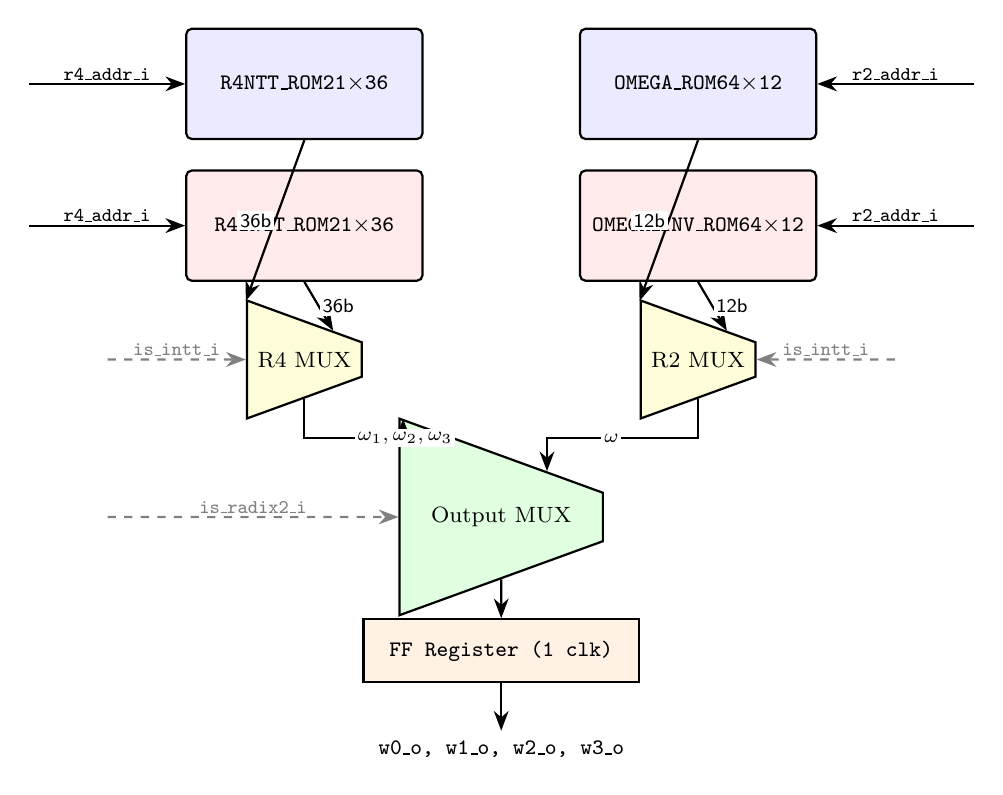
\begin{tikzpicture}[
    romblock/.style={draw, thick, minimum width=3cm, minimum height=1.4cm, rounded corners=2pt, font=\footnotesize\ttfamily},
    mux/.style={draw, thick, trapezium, trapezium angle=70, minimum width=1.5cm, minimum height=0.8cm, font=\footnotesize},
    arr/.style={-{Stealth[length=2.5mm]}, thick},
    label/.style={font=\scriptsize\sffamily, fill=white, inner sep=1pt}
]
    % ROMs
    \node[romblock, fill=blue!8]  (r4ntt)  at (0, 3)    {R4NTT\_ROM\\21$\times$36};
    \node[romblock, fill=red!8]   (r4intt) at (0, 1.2)  {R4INTT\_ROM\\21$\times$36};
    \node[romblock, fill=blue!8]  (omega)  at (5, 3)     {OMEGA\_ROM\\64$\times$12};
    \node[romblock, fill=red!8]   (omginv) at (5, 1.2)   {OMEGA\_INV\_ROM\\64$\times$12};

    % Muxes
    \node[mux, fill=yellow!15, shape border rotate=270] (r4mux) at (0, -0.5) {R4 MUX};
    \node[mux, fill=yellow!15, shape border rotate=270] (r2mux) at (5, -0.5) {R2 MUX};

    % Output mux
    \node[mux, fill=green!12, shape border rotate=270, minimum width=2.5cm] (outmux) at (2.5, -2.5) {Output MUX};

    % Connections: ROMs to muxes
    \draw[arr] (r4ntt.south) -- (r4mux.north west) node[label, midway, left] {36b};
    \draw[arr] (r4intt.south) -- (r4mux.north east) node[label, midway, right] {36b};
    \draw[arr] (omega.south) -- (r2mux.north west) node[label, midway, left] {12b};
    \draw[arr] (omginv.south) -- (r2mux.north east) node[label, midway, right] {12b};

    % Select signals
    \draw[arr, dashed, gray] (-2.5, -0.5) -- (r4mux.west) node[label, midway, above] {\port{is\_intt\_i}};
    \draw[arr, dashed, gray] (7.5, -0.5) -- (r2mux.east) node[label, midway, above] {\port{is\_intt\_i}};

    % Muxes to output mux
    \draw[arr] (r4mux.south) -- ++(0,-0.5) -| (outmux.north west) node[label, near start, right] {$\omega_1,\omega_2,\omega_3$};
    \draw[arr] (r2mux.south) -- ++(0,-0.5) -| (outmux.north east) node[label, near start, left] {$\omega$};

    % Select signal for output mux
    \draw[arr, dashed, gray] (-2.5, -2.5) -- (outmux.west) node[label, midway, above] {\port{is\_radix2\_i}};

    % Output register
    \node[draw, thick, minimum width=3.5cm, minimum height=0.8cm, fill=orange!10, font=\footnotesize\ttfamily] (reg) at (2.5, -4.2) {FF Register (1 clk)};
    \draw[arr] (outmux.south) -- (reg.north);

    % Outputs
    \draw[arr] (reg.south) -- ++(0, -0.6) node[below, font=\footnotesize\ttfamily] {w0\_o, w1\_o, w2\_o, w3\_o};

    % Address inputs
    \draw[arr] (-3.5, 3) -- (r4ntt.west) node[label, midway, above] {\port{r4\_addr\_i}};
    \draw[arr] (-3.5, 1.2) -- (r4intt.west) node[label, midway, above] {\port{r4\_addr\_i}};
    \draw[arr] (8.5, 3) -- (omega.east) node[label, midway, above] {\port{r2\_addr\_i}};
    \draw[arr] (8.5, 1.2) -- (omginv.east) node[label, midway, above] {\port{r2\_addr\_i}};
\end{tikzpicture}
\caption{Internal architecture of \sv{tf\_rom}.}
\label{fig:tf-rom-arch}
\end{figure}

\subsection{ROM Selection Logic}

The module uses two levels of multiplexing:

\paragraph{Level 1: Mode Selection (\port{is\_intt\_i}).}
\begin{align}
  \texttt{r4\_data} &=
  \begin{cases}
    \texttt{R4NTT\_ROM}[\texttt{r4\_addr\_i}]  & \text{if } \texttt{is\_intt\_i} = 0 \\
    \texttt{R4INTT\_ROM}[\texttt{r4\_addr\_i}] & \text{if } \texttt{is\_intt\_i} = 1
  \end{cases} \\[6pt]
  \texttt{r2\_data} &=
  \begin{cases}
    \texttt{OMEGA\_ROM}[\texttt{r2\_addr\_i}]      & \text{if } \texttt{is\_intt\_i} = 0 \\
    \texttt{OMEGA\_INV\_ROM}[\texttt{r2\_addr\_i}] & \text{if } \texttt{is\_intt\_i} = 1
  \end{cases}
\end{align}

\paragraph{Level 2: Pass Type Selection (\port{is\_radix2\_i}).}
\begin{align}
  (\texttt{w0\_o},\; \texttt{w1\_o},\; \texttt{w2\_o}) &=
  \begin{cases}
    (\texttt{r4\_w2},\; \texttt{r4\_w1},\; \texttt{r4\_w3}) & \text{if Radix-4} \\
    (\texttt{r2\_data},\; 0,\; 0)                             & \text{if Radix-2}
  \end{cases}
\end{align}

\paragraph{Output port mapping for Radix-4 mode:}

\begin{center}
\renewcommand{\arraystretch}{1.2}
\begin{tabular}{lccc}
\toprule
\textbf{Output} & \textbf{ROM field} & \textbf{Bit range} & \textbf{Role} \\
\midrule
\port{w0\_o} & $\omega_2$ & $[23:12]$ & Stage~B twiddle \\
\port{w1\_o} & $\omega_1$ & $[35:24]$ & Stage~A top \\
\port{w2\_o} & $\omega_3$ & $[11:0]$  & Stage~A bottom \\
\port{w3\_o} & (fixed)    & ---       & $\omega_4$ or $\omega_4^{-1}$ \\
\bottomrule
\end{tabular}
\end{center}

Note the \textbf{re-ordering}: the ROM stores $\{\omega_1, \omega_2, \omega_3\}$, but the outputs map $\omega_2 \to$ \port{w0}, $\omega_1 \to$ \port{w1}, $\omega_3 \to$ \port{w2}. This matches the PE datapath expectations where PE0 (connected to \port{w0}) performs the Stage~B multiplication.

\subsection{Read Latency}

All outputs are registered in a single \sv{always\_ff} block:
\begin{equation}
  \text{Read Latency} = 1 \text{ clock cycle}
\end{equation}

This means the address presented at cycle $n$ produces valid output at cycle $n+1$. The address generator must account for this pipeline delay.

% =====================================================================
\section{Module: \sv{tf\_addr\_gen} --- Twiddle Factor Address Generator}
\label{sec:tf-addr-gen-module}
% =====================================================================

\subsection{Port Interface}

\begin{center}
\renewcommand{\arraystretch}{1.3}
\begin{tabular}{lclcp{7cm}}
  \toprule
  \textbf{Port} & \textbf{Dir} & \textbf{Type} & \textbf{Width} & \textbf{Description} \\
  \midrule
  \port{clk}          & in  & \sv{logic}    & 1  & System clock \\
  \port{rst}          & in  & \sv{logic}    & 1  & Synchronous active-high reset \\
  \port{start\_i}     & in  & \sv{logic}    & 1  & Start pulse (1 cycle) \\
  \port{mode\_i}      & in  & \sv{pe\_mode\_e}& 2 & NTT / INTT / CWM \\
  \midrule
  \port{r4\_addr\_o}  & out & \sv{logic}    & 5  & $\to$ \port{tf\_rom.r4\_addr\_i} \\
  \port{r2\_addr\_o}  & out & \sv{logic}    & 6  & $\to$ \port{tf\_rom.r2\_addr\_i} \\
  \port{is\_intt\_o}  & out & \sv{logic}    & 1  & $\to$ \port{tf\_rom.is\_intt\_i} \\
  \port{is\_radix2\_o}& out & \sv{logic}    & 1  & $\to$ \port{tf\_rom.is\_radix2\_i} \\
  \port{valid\_o}     & out & \sv{logic}    & 1  & Addresses are valid \\
  \port{busy\_o}      & out & \sv{logic}    & 1  & Generator is active \\
  \port{pass\_o}      & out & \sv{logic}    & 2  & Current pass (0--3) \\
  \bottomrule
\end{tabular}
\end{center}

\subsection{FSM State Diagram}

\begin{figure}[H]
\centering
\begin{tikzpicture}[
    state/.style={draw, thick, rounded rectangle, minimum width=2.2cm, minimum height=0.8cm, font=\footnotesize\sffamily\bfseries},
    arr/.style={-{Stealth[length=2.5mm]}, thick},
    cond/.style={font=\scriptsize\sffamily, fill=white, inner sep=2pt}
]
    \node[state, fill=gray!15]   (idle) at (0,0)    {S\_IDLE};
    \node[state, fill=blue!12]   (p1)   at (3.5,0)  {S\_PASS\_1};
    \node[state, fill=blue!18]   (p2)   at (7,0)    {S\_PASS\_2};
    \node[state, fill=blue!24]   (p3)   at (10.5,0) {S\_PASS\_3};
    \node[state, fill=blue!30]   (p4)   at (10.5,-2.5){S\_PASS\_4};

    \draw[arr] (idle) -- (p1) node[cond, midway, above] {\port{start\_i}};
    \draw[arr] (p1)   -- (p2) node[cond, midway, above] {\textit{pass\_last}};
    \draw[arr] (p2)   -- (p3) node[cond, midway, above] {\textit{pass\_last}};
    \draw[arr] (p3)   -- (p4) node[cond, midway, right] {\textit{pass\_last}};
    \draw[arr] (p4)   -- ++(0,-1.2) -| (idle.south) node[cond, near start, right] {\textit{pass\_last}};

    % CWM shortcut
    \draw[arr, dashed, cwmgreen] (p1.south) -- ++(0,-0.8) -| (idle.south west) node[cond, near start, right] {\textit{CWM: pass\_last}};

    % Self loops (implied)
    \draw[arr, gray] (p1.north) to[loop above, looseness=5] node[cond] {counting} (p1.north);
    \draw[arr, gray] (p2.north) to[loop above, looseness=5] node[cond] {counting} (p2.north);
\end{tikzpicture}
\caption{FSM state diagram of \sv{tf\_addr\_gen}. CWM mode exits after Pass~1.}
\label{fig:fsm}
\end{figure}

\subsection{Internal Counters}

The module maintains four counters:

\begin{center}
\renewcommand{\arraystretch}{1.3}
\begin{tabular}{lccl}
  \toprule
  \textbf{Counter} & \textbf{Width} & \textbf{Reset} & \textbf{Behaviour} \\
  \midrule
  \sv{bf\_cnt\_r}    & 6 bits & Per-block  & Counts butterflies within a block \\
  \sv{block\_cnt\_r} & 6 bits & Per-pass   & Counts blocks within a pass \\
  \sv{r4\_cnt\_r}    & 5 bits & On start   & Sequential R4 ROM counter (\textbf{persists across passes}) \\
  \sv{r2\_cnt\_r}    & 6 bits & Per-pass   & Sequential R2 ROM counter \\
  \bottomrule
\end{tabular}
\end{center}

\paragraph{Critical detail: \sv{r4\_cnt\_r} persistence.}
The Radix-4 ROM counter is \emph{not} reset between passes. It starts at 0 when \port{start\_i} fires and counts continuously from 0 to 20 across all three Radix-4 passes:
\begin{itemize}
  \item NTT: Pass~1 uses $t=0$, Pass~2 uses $t=1..4$, Pass~3 uses $t=5..20$
  \item INTT: Pass~2 uses $t=0..15$, Pass~3 uses $t=16..19$, Pass~4 uses $t=20$
\end{itemize}

\subsection{Pass Configuration: Blocks and Butterflies}

Each state decodes a fixed pair $(\text{blocks\_max}, \text{bfs\_max})$ based on mode:

\begin{center}
\renewcommand{\arraystretch}{1.15}
\begin{tabular}{ll|cc|cc}
  \toprule
  & & \multicolumn{2}{c|}{\textbf{NTT}} & \multicolumn{2}{c}{\textbf{INTT}} \\
  \textbf{State} & \textbf{Pass} & blocks\_max & bfs\_max & blocks\_max & bfs\_max \\
  \midrule
  \sv{S\_PASS\_1} & 1 & 0 (R4, 1 blk)   & 63 (64 BFs) & 63 (R2, 64 blks) & 1 (2 BFs) \\
  \sv{S\_PASS\_2} & 2 & 3 (R4, 4 blks)   & 15 (16 BFs) & 15 (R4, 16 blks) & 3 (4 BFs) \\
  \sv{S\_PASS\_3} & 3 & 15 (R4, 16 blks) & 3 (4 BFs)   & 3 (R4, 4 blks)   & 15 (16 BFs) \\
  \sv{S\_PASS\_4} & 4 & 63 (R2, 64 blks) & 1 (2 BFs)   & 0 (R4, 1 blk)    & 63 (64 BFs) \\
  \bottomrule
\end{tabular}
\end{center}

Observe the \textbf{mirror symmetry}: NTT and INTT have exactly reversed pass structures.

\subsection{Counter Increment Logic}

The counting hierarchy operates as a nested loop:

\begin{enumerate}
  \item \textbf{Inner loop (butterflies):} \sv{bf\_cnt\_r} increments every clock cycle.
  \item \textbf{Outer loop (blocks):} When \sv{bf\_cnt\_r} reaches \sv{bfs\_max}:
    \begin{itemize}
      \item Reset \sv{bf\_cnt\_r} to 0
      \item Increment \sv{block\_cnt\_r}
      \item Increment the appropriate ROM counter:
        \begin{itemize}
          \item Radix-4 pass: increment \sv{r4\_cnt\_r}
          \item Radix-2 pass: increment \sv{r2\_cnt\_r}
        \end{itemize}
    \end{itemize}
  \item \textbf{Pass transition:} When both \sv{bf\_cnt\_r} = \sv{bfs\_max} and \sv{block\_cnt\_r} = \sv{blocks\_max}:
    \begin{itemize}
      \item Reset \sv{bf\_cnt\_r}, \sv{block\_cnt\_r}, and \sv{r2\_cnt\_r}
      \item Advance the FSM state
      \item Do \textbf{not} reset \sv{r4\_cnt\_r}
    \end{itemize}
\end{enumerate}

\paragraph{ROM counter increment timing.}
The ROM counter increments at the \emph{block boundary} (when \sv{bf\_last} is true), not at every cycle. This means all butterflies within a single block read the same ROM address --- they share the same twiddle factor, which is the correct behavior for the NTT butterfly structure.

% =====================================================================
\section{Address Output Routing}
\label{sec:addr-routing}
% =====================================================================

The combinational output logic selects which counter drives which ROM address bus:

\begin{center}
\renewcommand{\arraystretch}{1.3}
\begin{tabular}{l|cc}
  \toprule
  \textbf{Condition} & \port{r4\_addr\_o} & \port{r2\_addr\_o} \\
  \midrule
  Idle                  & 0          & 0                  \\
  CWM mode              & 0          & \sv{block\_cnt\_r} \\
  Radix-2 pass          & 0          & \sv{r2\_cnt\_r}    \\
  Radix-4 pass          & \sv{r4\_cnt\_r} & 0             \\
  \bottomrule
\end{tabular}
\end{center}

% #########################################################################
\part{Usage Guide: Connecting the Modules}
% #########################################################################

% =====================================================================
\section{Top-Level Wiring}
\label{sec:wiring}
% =====================================================================

\subsection{Connection Diagram}

\begin{figure}[H]
\centering
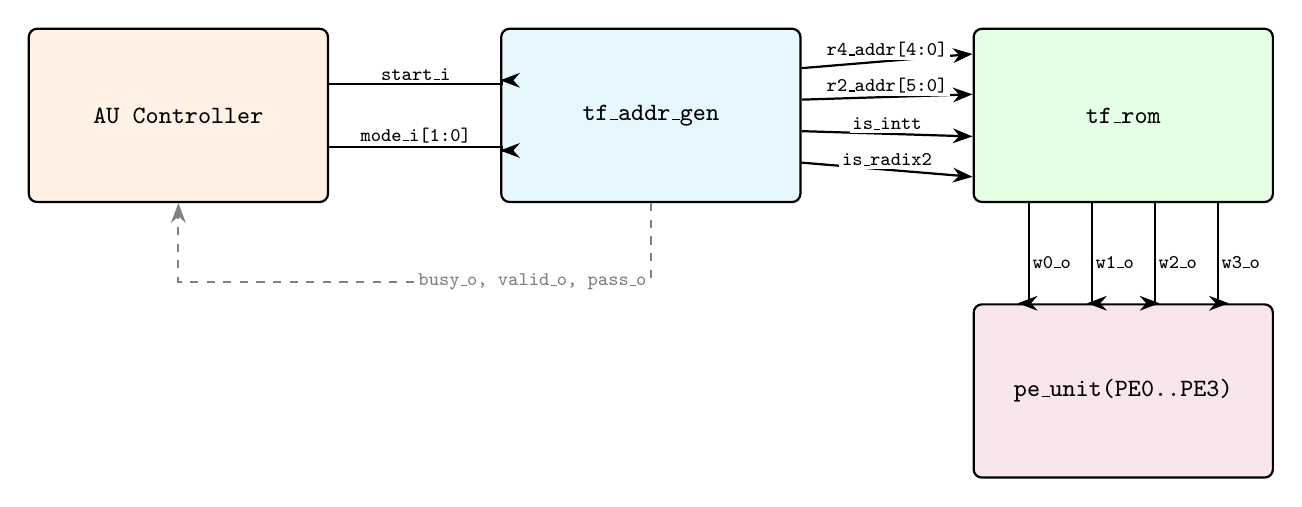
\begin{tikzpicture}[
    block/.style={draw, thick, minimum width=3.8cm, minimum height=2.2cm, rounded corners=3pt, font=\small\ttfamily},
    port/.style={font=\scriptsize\ttfamily},
    arr/.style={-{Stealth[length=2.5mm]}, thick},
    wire/.style={font=\scriptsize\ttfamily, fill=white, inner sep=1pt}
]
    % Blocks
    \node[block, fill=orange!10] (ctrl) at (0, 0)   {AU Controller};
    \node[block, fill=cyan!10]   (addr) at (6, 0)   {tf\_addr\_gen};
    \node[block, fill=green!10]  (rom)  at (12, 0)  {tf\_rom};
    \node[block, fill=purple!10] (pe)   at (12, -3.5) {pe\_unit\\(PE0..PE3)};

    % Controller -> Addr Gen
    \draw[arr] (ctrl.east) ++(0, 0.4) -- ++(2.2, 0) node[wire, midway, above] {start\_i} |- (addr.west |- {$(addr.north)!0.3!(addr.south)$});
    \draw[arr] (ctrl.east) ++(0, -0.4) -- ++(2.2, 0) node[wire, midway, above] {mode\_i[1:0]} |- (addr.west |- {$(addr.north)!0.7!(addr.south)$});

    % Addr Gen -> ROM
    \draw[arr] (addr.east) ++(0, 0.6) -- node[wire, above] {r4\_addr[4:0]} (rom.west |- {$(rom.north)!0.15!(rom.south)$});
    \draw[arr] (addr.east) ++(0, 0.2) -- node[wire, above] {r2\_addr[5:0]} (rom.west |- {$(rom.north)!0.38!(rom.south)$});
    \draw[arr] (addr.east) ++(0, -0.2) -- node[wire, above] {is\_intt} (rom.west |- {$(rom.north)!0.62!(rom.south)$});
    \draw[arr] (addr.east) ++(0, -0.6) -- node[wire, above] {is\_radix2} (rom.west |- {$(rom.north)!0.85!(rom.south)$});

    % ROM -> PE
    \draw[arr] (rom.south) ++(- 1.2, 0) -- ++(0, -0.75) node[wire, right] {w0\_o} |- (pe.north -| {$(pe.west)!0.15!(pe.east)$});
    \draw[arr] (rom.south) ++(-0.4, 0) -- ++(0, -0.75) node[wire, right] {w1\_o} |- (pe.north -| {$(pe.west)!0.38!(pe.east)$});
    \draw[arr] (rom.south) ++(0.4, 0) -- ++(0, -0.75) node[wire, right] {w2\_o} |- (pe.north -| {$(pe.west)!0.62!(pe.east)$});
    \draw[arr] (rom.south) ++(1.2, 0) -- ++(0, -0.75) node[wire, right] {w3\_o} |- (pe.north -| {$(pe.west)!0.85!(pe.east)$});

    % Status back to controller
    \draw[arr, dashed, gray] (addr.south) -- ++(0, -1) -| (ctrl.south) node[wire, near start, right] {busy\_o, valid\_o, pass\_o};
\end{tikzpicture}
\caption{Top-level connection between AU Controller, \sv{tf\_addr\_gen}, \sv{tf\_rom}, and \sv{pe\_unit}.}
\label{fig:top-level}
\end{figure}

\subsection{SystemVerilog Instantiation}

\begin{lstlisting}
// Wires between addr_gen and rom
logic [4:0] tf_r4_addr;
logic [5:0] tf_r2_addr;
logic       tf_is_intt;
logic       tf_is_radix2;

tf_addr_gen u_tf_addr_gen (
    .clk         (clk),
    .rst         (rst),
    .start_i     (ctrl_start),      // From AU Controller
    .mode_i      (ctrl_mode),       // From AU Controller
    .r4_addr_o   (tf_r4_addr),      // -> tf_rom
    .r2_addr_o   (tf_r2_addr),      // -> tf_rom
    .is_intt_o   (tf_is_intt),      // -> tf_rom
    .is_radix2_o (tf_is_radix2),    // -> tf_rom
    .valid_o     (tf_valid),        // -> AU Controller
    .busy_o      (tf_busy),         // -> AU Controller
    .pass_o      (tf_pass)          // -> AU Controller
);

tf_rom u_tf_rom (
    .clk         (clk),
    .rst         (rst),
    .is_intt_i   (tf_is_intt),      // <- tf_addr_gen
    .is_radix2_i (tf_is_radix2),    // <- tf_addr_gen
    .r4_addr_i   (tf_r4_addr),      // <- tf_addr_gen
    .r2_addr_i   (tf_r2_addr),      // <- tf_addr_gen
    .w0_o        (pe_w0),           // -> pe_unit (PE0)
    .w1_o        (pe_w1),           // -> pe_unit (PE2 mul1)
    .w2_o        (pe_w2),           // -> pe_unit (PE2 mul2)
    .w3_o        (pe_w3)            // -> pe_unit (PE3)
);
\end{lstlisting}

% =====================================================================
\section{Timing Diagram: NTT Operation}
\label{sec:timing-ntt}
% =====================================================================

\subsection{Complete NTT Cycle Count}

\begin{center}
\renewcommand{\arraystretch}{1.3}
\begin{tabular}{cccccc}
  \toprule
  \textbf{Pass} & \textbf{Type} & \textbf{Blocks} & \textbf{BFs/Block} & \textbf{Cycles} & \textbf{R4 counter $t$} \\
  \midrule
  1 & Radix-4 & 1  & 64 & 64  & 0 \\
  2 & Radix-4 & 4  & 16 & 64  & 1--4 \\
  3 & Radix-4 & 16 & 4  & 64  & 5--20 \\
  4 & Radix-2 & 64 & 2  & 128 & --- \\
  \midrule
  \multicolumn{4}{r}{\textbf{Total NTT:}} & \textbf{320 cycles} & \\
  \bottomrule
\end{tabular}
\end{center}

\subsection{Cycle-by-Cycle Example: NTT Pass~2}

Pass~2 has 4~blocks of 16~butterflies each. The R4 counter increments at each block boundary:

\begin{center}
\renewcommand{\arraystretch}{1.15}
\begin{tabular}{ccccc}
  \toprule
  \textbf{Cycle} & \sv{block\_cnt} & \sv{bf\_cnt} & \sv{r4\_cnt} & \textbf{ROM reads} \\
  \midrule
  64  & 0 & 0  & 1 & $\omega_1\!=\!296,\; \omega_2\!=\!1062,\; \omega_3\!=\!1409$ \\
  65  & 0 & 1  & 1 & (same --- held for entire block) \\
  $\vdots$ & 0 & $\vdots$ & 1 & $\vdots$ \\
  79  & 0 & 15 & 1 & (last BF of block 0) \\
  80  & 1 & 0  & 2 & $\omega_1\!=\!1703,\; \omega_2\!=\!650,\; \omega_3\!=\!1063$ \\
  $\vdots$ & & & & \\
  127 & 3 & 15 & 4 & (last BF of block 3 --- pass complete) \\
  \bottomrule
\end{tabular}
\end{center}

\subsection{Pipeline Latency Consideration}

Due to the 1-cycle ROM read latency:

\begin{equation}
  \text{Twiddle available at PE inputs} = \text{Address cycle} + 1
\end{equation}

The AU controller must ensure coefficient data arrives at the PEs one cycle after the address is presented. In practice, both the coefficient memory and the twiddle ROM have the same 1-cycle latency, so they are naturally aligned.

% =====================================================================
\section{Timing Diagram: INTT Operation}
\label{sec:timing-intt}
% =====================================================================

\subsection{Complete INTT Cycle Count}

\begin{center}
\renewcommand{\arraystretch}{1.3}
\begin{tabular}{cccccc}
  \toprule
  \textbf{Pass} & \textbf{Type} & \textbf{Blocks} & \textbf{BFs/Block} & \textbf{Cycles} & \textbf{ROM counter} \\
  \midrule
  1 & Radix-2 & 64 & 2  & 128 & R2: 0--63 \\
  2 & Radix-4 & 16 & 4  & 64  & R4: 0--15 \\
  3 & Radix-4 & 4  & 16 & 64  & R4: 16--19 \\
  4 & Radix-4 & 1  & 64 & 64  & R4: 20 \\
  \midrule
  \multicolumn{4}{r}{\textbf{Total INTT:}} & \textbf{320 cycles} & \\
  \bottomrule
\end{tabular}
\end{center}

Note the mirror: INTT starts with Radix-2 (unwinding the finest NTT stage first), then proceeds with three Radix-4 passes.

% =====================================================================
\section{CWM (Coefficient-Wise Multiplication) Mode}
\label{sec:cwm}
% =====================================================================

In CWM mode, the address generator produces a simple block counter (0--63) on \port{r2\_addr\_o}. The ROM is typically not used for twiddle factors in CWM mode; instead, the \port{r2\_addr\_o} may be routed to a separate coefficient ROM or used as a general-purpose address. The FSM exits after a single pass of 64~cycles.

\begin{center}
\begin{tabular}{cccc}
\toprule
\textbf{Mode} & \textbf{Passes} & \textbf{Total Cycles} & \textbf{ROM Used} \\
\midrule
NTT  & 4 & 320 & R4NTT + OMEGA \\
INTT & 4 & 320 & OMEGA\_INV + R4INTT \\
CWM  & 1 & 64  & (external) \\
\bottomrule
\end{tabular}
\end{center}

% =====================================================================
\section{Complete Usage Checklist}
\label{sec:checklist}
% =====================================================================

\begin{enumerate}[label=\textbf{\arabic*.}]
  \item \textbf{Reset} the system: Assert \port{rst} for at least 1 cycle.

  \item \textbf{Set mode}: Place the desired mode on \port{mode\_i}:
    \begin{itemize}
      \item \sv{PE\_MODE\_NTT} for forward NTT
      \item \sv{PE\_MODE\_INTT} for inverse NTT
      \item \sv{PE\_MODE\_CWM} for coefficient-wise multiplication
    \end{itemize}

  \item \textbf{Pulse start}: Assert \port{start\_i} for exactly 1 cycle.

  \item \textbf{Wait for operation}: Monitor \port{busy\_o}. While high:
    \begin{itemize}
      \item \port{valid\_o} indicates valid addresses are being produced
      \item \port{pass\_o} indicates the current pass number (0--3)
      \item \port{is\_radix2\_o} indicates whether the current pass is Radix-2
      \item Twiddle factor outputs (\port{w0\_o}--\port{w3\_o}) are valid 1 cycle after addresses appear
    \end{itemize}

  \item \textbf{Completion}: When \port{busy\_o} deasserts, all 320 cycles (NTT/INTT) or 64 cycles (CWM) have completed. The system is ready for a new \port{start\_i} pulse.

  \item \textbf{PE connections}: Wire the four twiddle outputs to the PE array:
    \begin{itemize}
      \item \port{w0\_o} $\to$ PE0 (multiplier in butterfly)
      \item \port{w1\_o} $\to$ PE2, multiplier input 1
      \item \port{w2\_o} $\to$ PE2, multiplier input 2
      \item \port{w3\_o} $\to$ PE3 (fixed $\omega_4$ or $\omega_4^{-1}$)
    \end{itemize}
\end{enumerate}

% =====================================================================
\section{Summary of Key Design Decisions}
\label{sec:design-decisions}
% =====================================================================

\begin{enumerate}[label=\textbf{D\arabic*.}]
  \item \textbf{Four ROMs instead of one}: Separate NTT/INTT and R4/R2 ROMs eliminate runtime conditional logic and reduce multiplexer depth.

  \item \textbf{36-bit bundled words}: Three twiddle factors packed per word allow single-cycle fetch for all three Radix-4 PE multipliers.

  \item \textbf{Pre-negated INTT values}: Absorbing the sign flip into ROM constants eliminates a modular negation circuit from every INTT butterfly.

  \item \textbf{Sequential addressing ($t$++)}: Avoids complex bit-reversal address computation hardware. The Python script pre-computes the correct order offline.

  \item \textbf{Persistent R4 counter}: The \sv{r4\_cnt\_r} counter is not reset between Radix-4 passes, allowing it to smoothly index entries 0--20 across three passes without additional logic.

  \item \textbf{1-cycle registered outputs}: ROM outputs are registered for timing closure, naturally aligning with the coefficient memory pipeline.

  \item \textbf{Fixed $\omega_4$ on dedicated output}: PE3's twiddle factor never changes within a mode (NTT or INTT), so it is implemented as a simple registered mux rather than consuming a ROM port.
\end{enumerate}

\end{document}